\section{Конструкторский раздел}
В этом разделе выделяются требования к разрабатываемому методу.
Кратко описывается спроектированный метод и его особенности.
Описываются конфигурации нейронных сетей и датасет для их обучения.
Составляется структура программного комплекса, описывается взаимодействия отдельных частей системы. 

\subsection{Требования к разрабатываемому методу}
Метод очищения цветного изображения от импульсных шумов должен соответствовать следующим требованиям:
\begin{enumerate}
	\item Принимать на вход изображение в форматах JPG или JPEG, а также вид шума -- шум соли или перца. 
	Гарантируется, что процент шума на изображении не превышает 40\%.
	\item Очистить изображение от шумов.
	\item Вывести на экран результат работы алгоритма.
	\item Использовать в своей работе нейронные сети.
\end{enumerate}

\subsection{Требования к разрабатываемому программному комплексу}
Програмнный комплекс, реализующий интерфейс к разработанному методу, должен позволять выполнять следующие действия:
\begin{itemize}
	\item возможность загрузки изображений с помощью графического интерфейса;
	\item возможность выбора типа искомого шума: шум соли или шум перца;
	\item возможность просмотра результата работы метода и сравнения с исходным изображением.
\end{itemize}

\subsection{Проектирование метода удаления шумов}
Разработанный метод должен учитывать следующие особенности ранее известных алгоритмов:
\begin{enumerate}
	\item Метод медианной фильтрации позволяет очистить изображения от большинства проблемных пикселей, но искажает цветовую составляющую исходного изображения.
	\item Нейронная сеть RIDNET плохо справляется с импульсными шумами. 
	В случае обучения на картинках с импульсными шумами она подстраивается на определенный их процент, а обучать на все возможные проценты различные модели является нецелесообразным.
	\item Конфигурация нейронной сети RIDNET позволяет обучить ее для того, чтобы корректировать цвета пикселей, полученные в результате применения медианного фильтра.
\end{enumerate}

\subsubsection{Основной алгоритм работы}
Учитывая особенности известных методов, перечисленные ранее, был разработан метод, позволяющий бороться с шумами на изображениях.

В первую очередь, картинку требуется разбить на изображения небольшого размера, называющиеся патчами.
Это следует сделать для того, чтобы корректнее обучить нейронные сети и получить вменяемый результат.

Затем нужно оценить количество шума на патче.
В случае, если оно больше, чем некое пороговое значение, то требуется предварительно применить медианный фильтр.
Результаты работы медианного фильтра нужно обработать в нейронной сети, способной к коррекции исходных цветов изображений.
По итогу предварительный результат попадает на нейронную сеть, предназначенную для очистки изображения от шумов.

Для получения конечного результата требуется склеить изображение из патчей в нужной последовательности.

Схема алгоритма представлена на рисунке \ref{contruct::mainAlgo}:
\FloatBarrier
\begin{figure}[h]	
	\begin{center}
		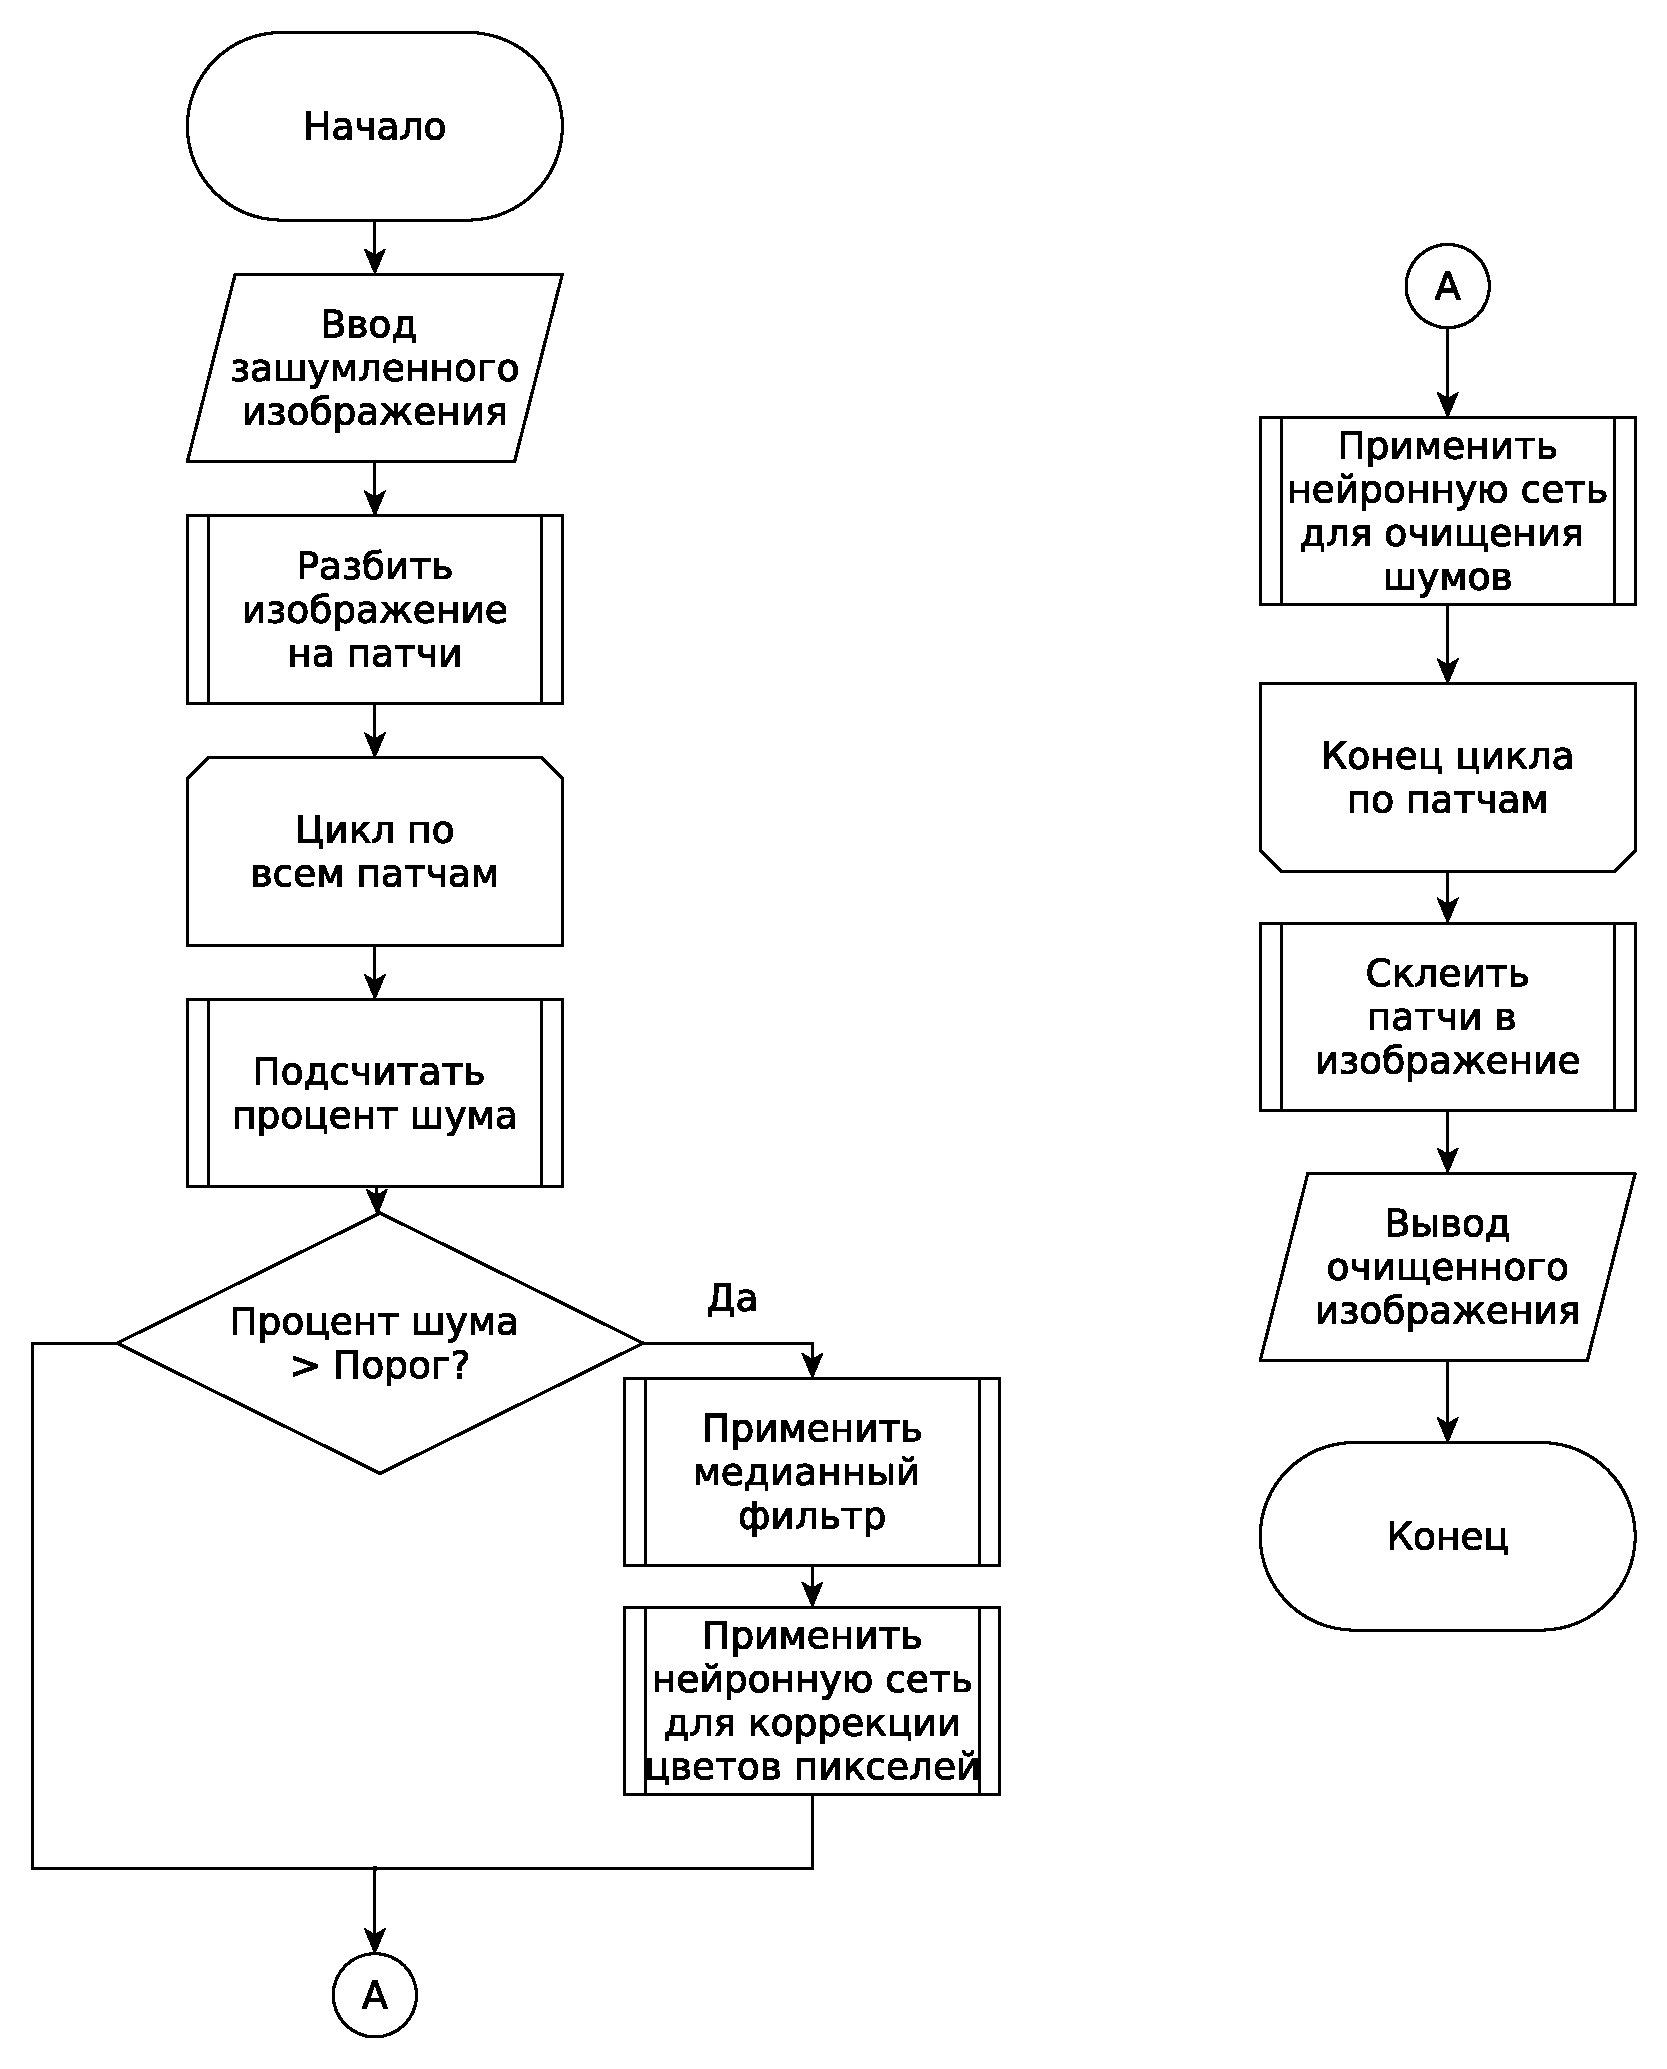
\includegraphics[width=\linewidth]{inc/pdf/mainAlgo.pdf}
	\end{center}
	\captionsetup{justification=centering}
	\caption{Верхнеуровневая схема алгоритма}
	\label{contruct::mainAlgo}
\end{figure}
\FloatBarrier

\subsubsection{Подсчет количества шумов в изображении}
Для принятия решения об использовании медианного фильтра требуется подсчитать, превышает ли количество импульсных шумов необходимый порог.

Все цвета пикселей делятся на следующие три категории:
\begin{enumerate}
	\item Цвета, принимающиеся за шум соли.
	\item Цвета, принимающиеся за шум перца.
	\item Цвета, не принимающиеся за шум.
\end{enumerate}

Однако главная сложность состоит в том, что пиксель может быть ошибочно принят за шум, если он находятся на фоне, соответствующим шуму.
Например, если рассматривать яркое небо, то почти все пиксели в этом случае можно интерпретировать как шум соли.
Соответственно, нужно учитывать контекст для принятия решения.

Для этого требуется оценить цвет рассматриваемого пикселя по сравнению с соседями.
Нужно подсчитать среднюю разницу цветов с соседними пикселями, в соответствии с сеткой, используемой в медианном фильтре.
Если она получается больше, чем заданная разница, то пиксель определяется как шум, иначе -- как исходный пиксель.
Заданная разница рассчитывается экспертной оценкой.

В результате требуется посчитать количество пикселей, принятых за шум. 
Так как размер патча заранее известен, достаточно найти отношения импульсного шума к общему число пикселей.

Схема алгоритма подсчета количества шумов представлена на рисунке \ref{contruct::count}:
\FloatBarrier
\begin{figure}[h]	
	\begin{center}
		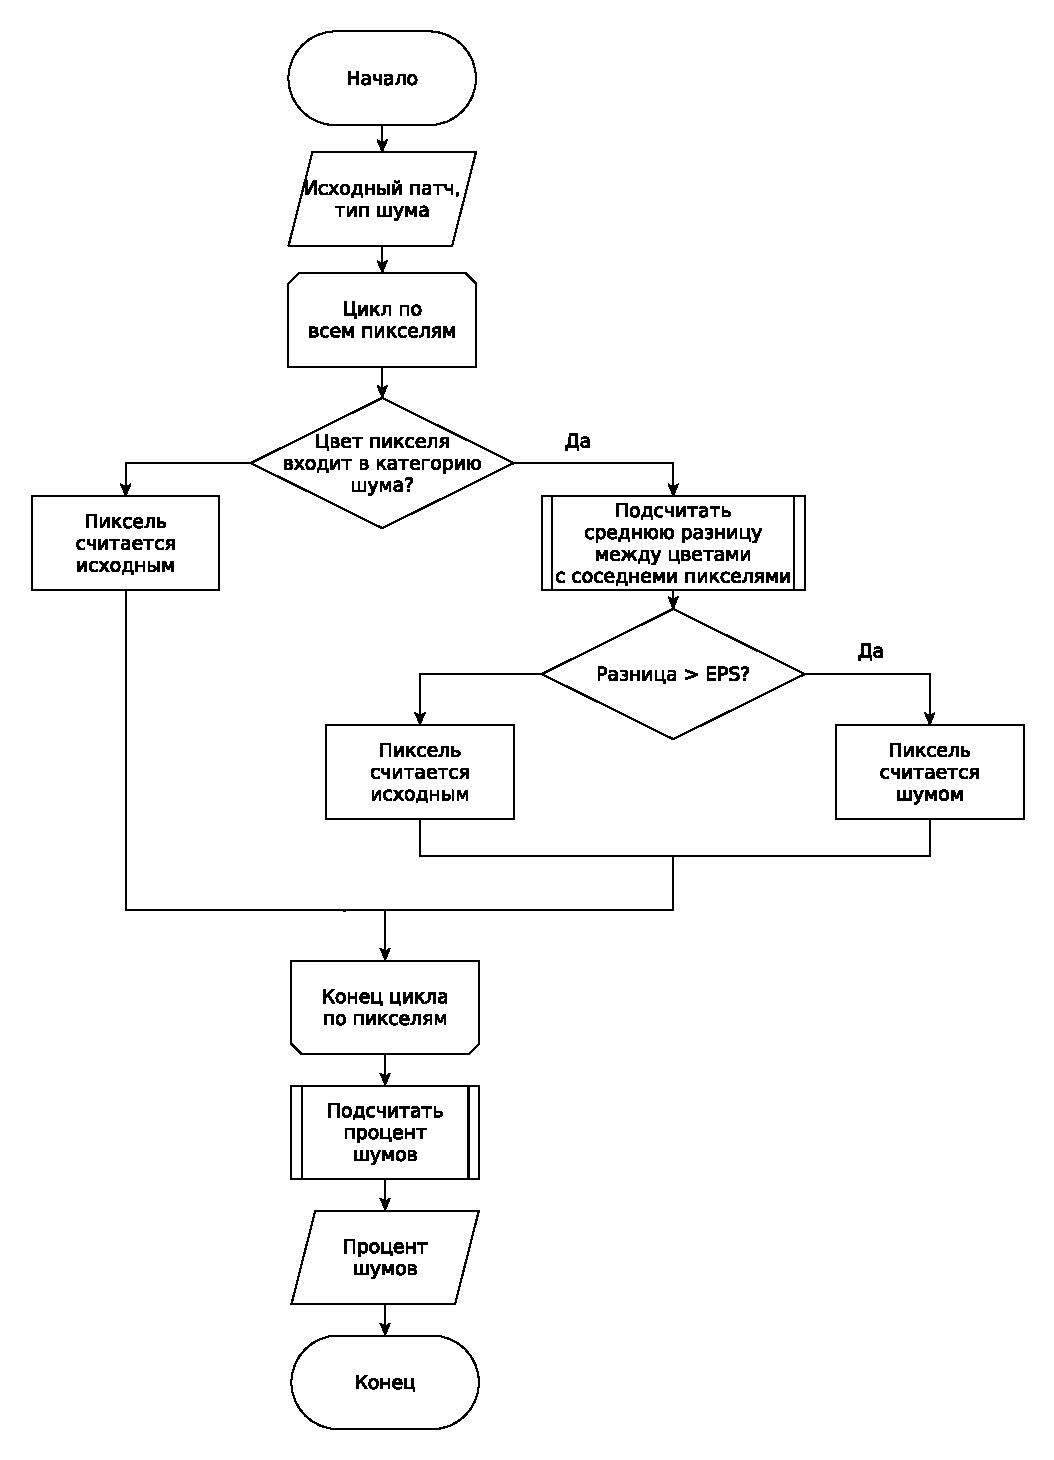
\includegraphics[width=\linewidth]{inc/pdf/shumCount.pdf}
	\end{center}
	\captionsetup{justification=centering}
	\caption{Схема алгоритма подсчета количества шумов}
	\label{contruct::count}
\end{figure}
\FloatBarrier

\subsubsection{Конфигурация нейронных сетей}
В качестве основы для итоговой конфигурации нейронной сети была выбрана модель RIDNET.

В нее были добавлены соответствующие изменения:
\begin{enumerate}
	\item Она состоит из трех EAM-модулей, а не из четырех, как в исходном алгоритме.
	\item В качестве функции активации выбрана сигмоида на всех элементах EAM-модуля, а не ReLu.
	\item Функция потерь -- среднеквадратичное отклонение от результата, а не абсолютная ошибка, как в RIDNET.
\end{enumerate}

Конфигурация нейронной сети для очищения изображения от шумов также основана на RIDNET, но в качестве функции активации внутри EAM-модуля использовалась сигмоида для частей, склеивающих результат с нескольких каналов в один выход.

В качестве функции оптимизации был использован Adam (адаптивная оценка момента).
Вместо того чтобы адаптировать скорость обучения параметров на основе среднего первого момента (среднего значения), Adam также использует среднее значение вторых моментов градиентов.

\subsubsection{Данные для обучения модели}
В качестве данных, используемых для обучения моделей, был использован датасет BSDS500, использующий для верификации алгоритмов, специализирующихся на очищении гауссовых шумов из изображений.
Выбор обусловлен тем, что он уже использовался для оценки качества работы других нейронных сетей, перечисленных в аналитическом разделе, соответственно, не придется дополнительно обучать другие модели и применять фильтры для сравнения результата.
Также множество изображений было составлено таким образом, что цветовая гамма изображений в них отличается, что позволит проверить метод в различных ситуациях.

Однако для моделирования импульсных шумов требуется разработать собственные функции.

\subsection{Структура разрабатываемого программного комплекса}
Разрабатываемый программный комплекс состоит из трех модулей:
\begin{enumerate}
	\item Модуль разработки и обучения нейронных сетей, в котором также происходит разработка датасета.
	\item Модуль обработки изображений.
	\item Модуль взаимодействия с пользователем.
\end{enumerate}

На рисунке \ref{contruct::module1} представлена схема модуля разработки и обучения нейронных сетей:
\FloatBarrier
\begin{figure}[h]	
	\begin{center}
		\includegraphics[width=\linewidth]{inc/pdf/module1.pdf}
	\end{center}
	\captionsetup{justification=centering}
	\caption{Схема модуля разработки и обучения нейронных сетей}
	\label{contruct::module1}
\end{figure}
\FloatBarrier

Валидация результата должна происходить по следующим правилам:
\begin{enumerate}
	\item Значение PSNR для очищенного изображения превышает показатель для загрязненного изображения.
	\item Значение PSNR больше, чем для реализации исходных алгоритмов: RIDNET и медианный фильтр.
\end{enumerate}

\newpage
Схема модуля взаимодействия с пользователем представлена на рисунке \ref{contruct::module2}:
\FloatBarrier
\begin{figure}[h]	
	\begin{center}
		\includegraphics[width=\linewidth]{inc/pdf/module2.pdf}
	\end{center}
	\captionsetup{justification=centering}
	\caption{Схема модуля взаимодействия с пользователем}
	\label{contruct::module2}
\end{figure}
\FloatBarrier

\subsection*{Выводы}
Были составлены требования к разрабатываемому методу.
Был спроектирован метод с учетом особенностей уже существующих способов, описаны его особенности, составлены схемы основных алгоритмов.
Была разработана конфигурация нейронных сетей, описан путь составления датасета для его обучения.
Была составлена структура программного комплекса, описаны взаимодействия отдельных частей системы.